\documentclass{article}

\usepackage{color, listings, bm, amsmath, blkarray}
% \usepackage[percent]{overpic}
% \usepackage{tikz,graphicx}
% \usepackage{graphicx}

\begin{document}
% todo:
% include snowmelt in model run. see if it's worth including with precip and temp as a climate predictor
% introduce terminology:
% responses = water temp, Q
% climatic predictors = air temp, precip, drought
% landscape predictors = many
%include hydrograph figures from kathy liederman and julian olden to show
    %rain dom, rain and snow, snow dom
%include the over-time plots in the supplemental information

\section*{Introduction}

\section*{Methods}

\subsection*{Study region}

I'll probably mention anything relevant to this in the intro.

\subsection*{Water and climate data}

The two response variables used in our analyses were water temperature and discharge. We obtained monthly water temperature readings from 1978 through 2015 via the Washington Department of Ecology's River and Stream Water Quality Monitoring program \colorbox{red}{\lstinline{cite}}. In all, 24 monitoring sites within the Puget Sound region (Fig. \colorbox{red}{\lstinline{1}}) were included, representing 19 rivers across 9 counties, and ranging from 4 to 775 m in elevation. For one site at each river, monthly discharge time series were available, either for the same location as one of the temperature monitoring sites, or for another location within 30 km on the same major reach. Discharge data were aggregated by monthly mean from the USGS Washington Water Science Center (collected daily 1978-2007) and the USGS National Water Information System (collected at 15-minute intervals 2008-2015). At least one discharge monitoring site was available for every river represented in the temperature dataset.

Potential climatic predictors of water temperature and discharge included mean and max air temperature, total precipitation, snowmelt, and hydrologic drought, averaged by month across the response variable time series. All but snowmelt are available through the U.S. Climate Divisional Dataset, developed by the National Centers for Environmental Information (NCEI)\colorbox{red}{\lstinline{cite}}. We acquired climatic predictor data grouped by Washington State climate division, and all but two of our sites fell within divisions 3 (Puget Sound Lowland) and 4 (East Olympic/Cascade Foothills). We therefore aggregated these data by monthly mean across the two regions (after verifying their post-standardization similarity), resulting in a single dataset of four regional, climatic predictors. A snowmelt time series was then added to this dataset, using monthly mean records from six SNOTEL sites (Bumping Ridge, Elbow Lake, Mount Crag, Park Creek Ridge, Stevens Pass, White Pass) listed by the USDA's Natural Resources Conservation Service \colorbox{red}{\lstinline{cite}}. We calculated monthly snowmelt for each site as the absolute value of negative differences in cumulative snow water equivalent from each month to the next. The snowmelt time series was assigned zeros for any positive differences (accumulations). 

%More information on all datasets can be found in \colorbox{red}{\lstinline{Appendix A}}. 

\subsection*{Time series analysis}

Response time series were modeled using dynamic factor analysis (DFA; \colorbox{red}{\lstinline{Zuur et al. 2003}}), a multivariate technique that can be thought of as an analog to principal component analysis in the time domain. In DFA, response time series are fit with a linear combination of shared, random-walk trends (usually many fewer than the total number of response series), predictors (which can have unique effects on each response series), and random error. We chose DFA over a traditional multivariate state space approach for two reasons. First, it provides advantages in computational efficiency, as 1-5 shared trends often adequately capture variation across dozens of responses, and at much lower parameter cost. Second, in terms of identifying what drives the shared trends, having fewer of them allows for greater inferential parsimony. Being a multivariate technique, DFA also provides an advantage over univariate alternatives in that covariance structure among responses can be specified and compared. All models were fit using maximum likelihood estimation by automatic differentiation, with Template Model Builder software \colorbox{red}{\lstinline{Kristensen et al. 2015}}, which we called using package TMB in R \colorbox{red}{\lstinline{R Core team 2016...}}.

DFA takes the following form:

\begin{equation}
    \textbf{x}_t = \textbf{x}_{t-1} + \textbf{w}_t\textrm{, where } \textbf{w}_t \sim \textrm{MVN}(0,\textbf{Q})
\end{equation}
\begin{equation}
    \textbf{y}_t = \textbf{Zx}_t + \textbf{Dd}_t + \textbf{v}_t\textrm{, where } \textbf{v}_t \sim \textrm{MVN}(0,\textbf{R})
\end{equation}
\begin{equation}
    \textbf{x}_0 \sim \textrm{MVN}(0,\bm{\Lambda})
\end{equation}

At time step {\it t}, the $m \times 1$ vector of shared trends (\textbf{x}) is a function of \textbf{x} in the previous step, plus normal error (\textbf{w}; $m\times 1$; Eq. 1). This is the definition of a random walk. The $n\times 1$ response vector (\textbf{y}) at time {\it t} is a function of the shared trends and their factor loadings (\textbf{Z}; $n\times m$), covariates (\textbf{d}; $q\times 1$) and their river-specific effects (\textbf{D}; $n\times q$), and a second normal error term (\textbf{v}; $n\times 1$; Eq. 2). \textbf{R} and \textbf{Q} are variance-covariance matrices of order m, and \textbf{Q} is set to identity for model identifiability (\colorbox{red}{\lstinline{Harvey 1989}}). The initial state of the shared trend vector ($\bm{x}_0$) is multivariate-normally distributed with a mean of zero and a diagonal variance-covariance matrix with large variance (e.g. 5; Eq. 3). Response and predictor data were standardized to facilitate comparison of effect sizes and avoid error inflation.

% Response data were centered on 0, but not scaled, to avoid error inflation \colorbox{red}{\lstinline{details and citation}}.

Because we were interested in isolating the effects of climatic predictors on river temperature and discharge, we used fixed factors to absorb recurring seasonal variation not related to the predictors, with one factor level for each month. These factors were incorporated into the covariate matrix (\textbf{d}). Thus, the coefficient in \textbf{D} relating, say, air temperature (predictor) and water temperature (response), represents the effect size of the former on the latter. In other words, it is the change in water temperature accompanying a unit change in air temperature across the whole time series. We call this relationship "coupling." We were also interested in coupling by month for specific predictors, which required that the focal predictor in a particular model be arranged seasonally. Concretely,

$$
\textbf{d} = \begin{blockarray}{cccccc}
& \textrm{Jan}_{1978} & \textrm{Feb}_{1978} & \textrm{Mar}_{1978} & \cdots & \textrm{Dec}_{2015} \\
\begin{block}{c(ccccc)}
    1 & 1 & 0 & 0 & \cdots & 0 \\
    2 & 0 & 1 & 0 & \cdots & 0 \\
    3 & 0 & 0 & 1 & \cdots & 0 \\
      & \vdots & \vdots & \vdots & \ddots & \vdots \\
    12 & 0 & 0 & 0 & \cdots & 1 \\
    13 & \theta_{precip}^{(1)} & \theta_{precip}^{(2)} & \theta_{precip}^{(3)} & \cdots & \theta_{precip}^{(T)} \\
    14 & \theta_{air}^{(1)} & 0 & 0 & \cdots & 0 \\
    15 & 0 & \theta_{air}^{(2)} & 0 & \cdots & 0 \\
    16 & 0 & 0 & \theta_{air}^{(3)} & \cdots & 0 \\
      & \vdots & \vdots & \vdots & \ddots & \vdots \\
    25 & 0 & 0 & 0 & \cdots & \theta_{air}^{(T)} \\
\end{block}
\end{blockarray}
$$

is the covariate matrix structure necessary to account for exogenous seasonal variation (rows 1-12), and overall effect of precipitation (row 13), while also yielding the by-month effect of air temperature (rows 13-24) on the response (\textbf{y}).

Additional, non seasonal variation due to exogenous effects loads onto the shared trends, and a portion of remaining variation is absorbed by error matrix \textbf{v}. We fit models using four unique error structures (\textbf{R}), to allow for different suites of unknown drivers affecting rivers. We included shared variance and zero covariance, individual variance and zero covariance, shared variance and shared covariance, and unconstrained error. Details on these structures and their implications can be found in colorbox{red}{\lstinline{Holmes et al. (2012)}}. The best models for water temperature and discharge were determined with AIC.

\subsection*{Landscape predictors and post-hoc regression}

After model selection, climatic predictor effect sizes for each river were back-transformed to their original scales and regressed against landscape predictors in order to identify possible watershed-scale controls on coupling. To achieve this, we amassed an additional dataset of landscape features. These were collected individually for each of the watersheds corresponding to our 24 river sites, using the EPA's StreamCat (stream-catchment) data library \colorbox{red}{\lstinline{cite}} and the National Hydrography Dataset (NHDPlusV2)\colorbox{red}{\lstinline{cite}}. Each site was mapped to an individual river reach, defined as a segment bounded on each end by a stream or river source, confluence, or mouth. The region contributing flow to this reach (its watershed) was then fetched, along with selected areal data, from the NHDPlusV2 database. Landscape attributes used as predictors were aggregated by watershed mean where applicable, and include elevation (m), total area (km\textsuperscript{2}), base flow index, soil permeability (cm hr\textsuperscript{-1}), water table depth (cm), bedrock depth (cm), Base Flow Index (BFI; \%), runoff (mm mo\textsuperscript{-1}), percent ice and snow (National Land Cover Database [NLDC] 2006 and 2011 average), riparian population density (people km\textsuperscript{-2} within 100m of streams; 2010 census), riparian road density (km km\textsuperscript{-2}; 2010 census), and percent riparian urban land (NLCD 2011). We also calculated area over 1000 m (km\textsuperscript{2}) and mean slope (percent rise) by delineating watersheds from a digital elevation model in ArcMap \colorbox{red}{\lstinline{cite}}.

\section*{Results}

% \begin{overpic}[grid,scale=0.5,unit=1mm]{figures/16_temp_all_reg.pdf}
% \begin{overpic}[width=1\textwidth,grid,tics=10]{figures/16_temp_all_reg.pdf}
% \put (1,55) {\small
% chili chili chili chili chili chili chili chili chili chili chili chili chili chili
% chili chili chili chili chili chili chili chili chili chili chili chili chili chili\\
% chili chili chili chili chili chili chili chili chili chili chili chili chili chili\\
% chili chili chili chili chili chili chili chili chili chili chili chili chili chili\\
% chili chili chili chili chili chili chili chili chili chili chili chili chili chili\\
% chili chili chili chili chili chili chili chili chili chili chili chili chili chili
% }
% \end{overpic}

% \begin{tikzpicture}
% \node (img) {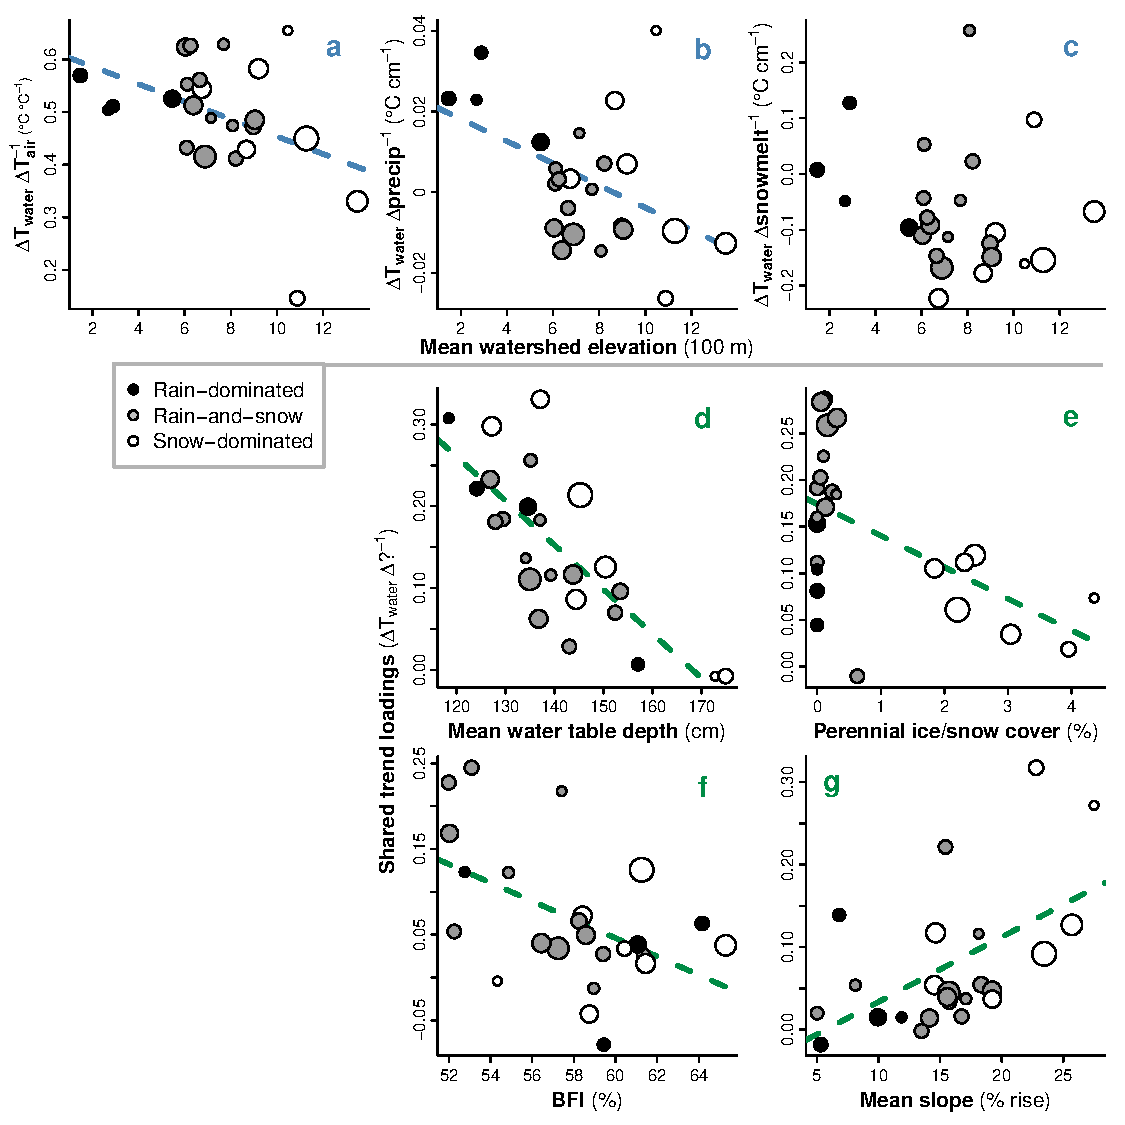
\includegraphics[width=1\textwidth]{figures/16_temp_all_reg.pdf}};
% \node [below left,text width=4cm,align=left] at (img.north east){\small Lorem ipsum dolor sit amet consectetur and then a bunch more stuff that no one remembers.};
% \end{tikzpicture}

\begin{picture}(100,100)
\put(.1,.1){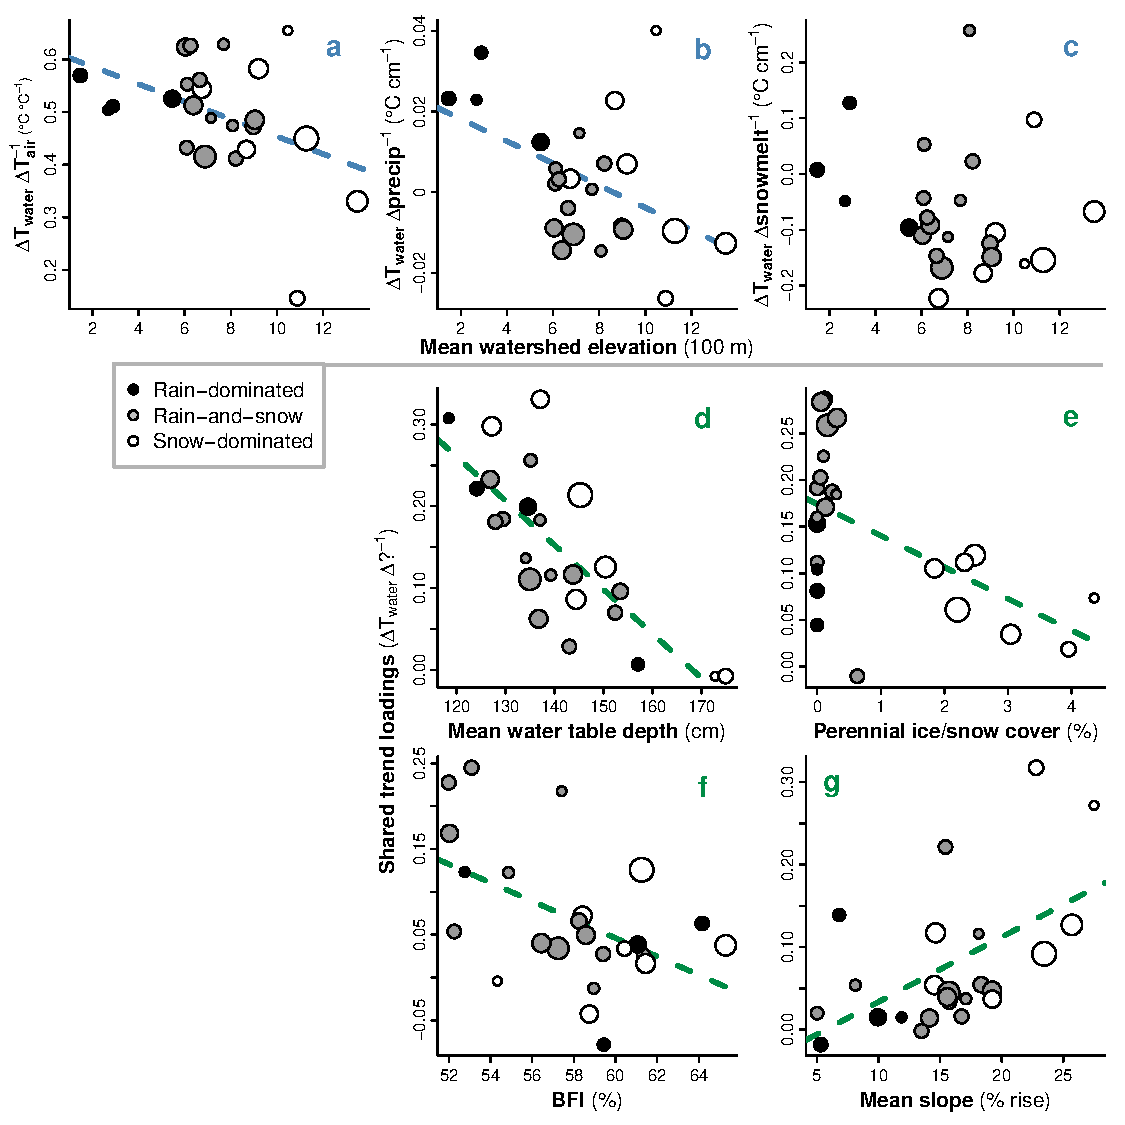
\includegraphics{figures/16_temp_all_reg.pdf}}
% \put(.01\textwidth,.3\textwidth){hello}
\end{picture}

% \begin{figure}
%   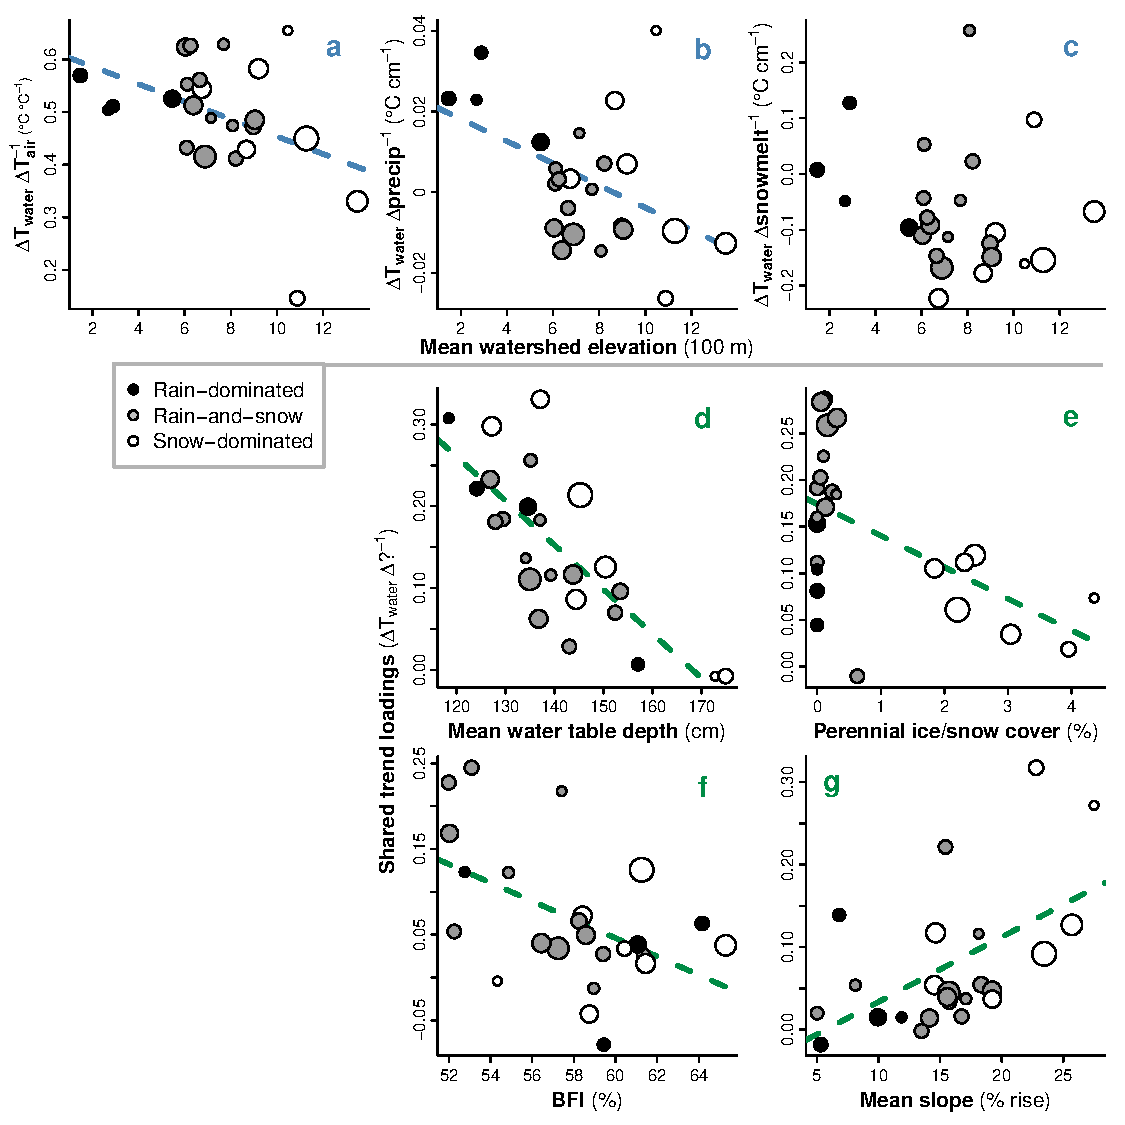
\includegraphics[width=\linewidth]{figures/16_temp_all_reg.pdf}
%   \caption{A boat.}
%   \label{fig:boat1}
% \end{figure}

\end{document}



% https://wa.water.usgs.gov/data/realtime/adr/interactive/ #discharge daily
% https://waecy.maps.arcgis.com/apps/Viewer/index.html?appid=832e254169e640fba6e117780e137e7b #Q 15min
% http://www.horizon-systems.com/NHDPlus/NHDPlusV2_17.php #nhdplus
% ftp://newftp.epa.gov/EPADataCommons/ORD/NHDPlusLandscapeAttributes/StreamCat/HydroRegions/ #streamca
% ncdc.noaa.gov/cag/time-series/us #climate data
% https://www.nrcs.usda.gov/wps/portal/nrcs/detail/or/snow/?cid=nrcs142p2_046350 #snow
% https://arxiv.org/pdf/1509.00660.pdf #TMB
% Harvey, A. C. 1989. Forecasting, structural time series models and the Kalman flter. Cambridge University Press, Cambridge, UK.
